%% Copyright (c) 2015-2020, RTE (http://www.rte-france.com)
%% See AUTHORS.txt
%% All rights reserved.
%% This Source Code Form is subject to the terms of the Mozilla Public
%% License, v. 2.0. If a copy of the MPL was not distributed with this
%% file, You can obtain one at http://mozilla.org/MPL/2.0/.
%% SPDX-License-Identifier: MPL-2.0
%% This file is part of Dynawo, an hybrid C++/Modelica open source time domain
%% simulation tool for power systems.
\documentclass[a4paper, 12pt]{report}

%%  Copyright (c) 2015-2019, RTE (http://www.rte-france.com)
%%  See AUTHORS.txt
%%  All rights reserved.
%%  This Source Code Form is subject to the terms of the Mozilla Public
%%  License, v. 2.0. If a copy of the MPL was not distributed with this
%%  file, you can obtain one at http://mozilla.org/MPL/2.0/.
%%  SPDX-License-Identifier: MPL-2.0
%%
%%  This file is part of Dynawo, an hybrid C++/Modelica open source time domain
%%  simulation tool for power systems.


%%%%%%%%%%%%%%%%%%%%%%%%%%%%%%%%%%%%%%%%%%%
% Define text and document settings
%%%%%%%%%%%%%%%%%%%%%%%%%%%%%%%%%%%%%%%%%%%

\usepackage{lmodern} % Latin Modern fam­ily of fonts
\usepackage[english]{babel} % English

% Specify encoding
\usepackage[utf8]{inputenc} % Input
\usepackage[T1]{fontenc} % Output

% Document structure setup
\usepackage{titlesec} % To change chapter format
\setcounter{tocdepth}{3} % Add subsubsection in Content
\setcounter{secnumdepth}{3} % Add numbering for subsubsection
\setlength{\parindent}{0pt} % No paragraph indentation

% Avoid numbering starting at each chapter for figures
\usepackage{chngcntr}
\counterwithout{figure}{chapter}

% Change title format for chapter
\titleformat{\chapter}{\Huge\bf}{\thechapter}{20pt}{\Huge\bf}

% To add links on page number in Content and hide red rectangle on links
\usepackage[hidelinks, linktoc=all]{hyperref}
\usepackage[nottoc]{tocbibind} % To add biblio in table of content
\usepackage{textcomp} % For single quote
\usepackage{url} % Allow linebreaks in \url command
\usepackage{listings} % To add code samples

% Define typography
\usepackage{xspace}
\usepackage{dirtree}
\newcommand{\Dynawo}[0]{Dyna$\omega$o\xspace}

% Default listings parameters
\lstset
{
  aboveskip={1\baselineskip}, % A bit of space above
  backgroundcolor=\color{shadecolor}, % Choose the background color
  basicstyle={\ttfamily\footnotesize}, % Use font and smaller size \small \footnotesize
  breakatwhitespace=true, % Sets if automatic breaks should only happen at whitespace
  breaklines=true, % Sets automatic line breaking
  columns=fixed, % Nice spacing -> fixed / flexible
  mathescape=false, % Escape to latex false
  numbers=left, % Where to put the line-numbers
  numberstyle=\tiny\color{gray}, % The style that is used for the line-numbers
  showstringspaces=false, % Do not emphasize spaces in strings
  tabsize=4, % Number of spaces of a TAB
  texcl=false, % Activates or deactivates LaTeX comment lines
  upquote=true % Upright quotes
}

%%%%%%%%%%%%%%%%%%%%%%%%%%%%%%%%%%%%%%%%%%%
% Define plots settings
%%%%%%%%%%%%%%%%%%%%%%%%%%%%%%%%%%%%%%%%%%%

% Macro pack­age for cre­at­ing graph­ics
\usepackage{tikz}
\usepackage{subfigure}
\usepackage{float}

% Draws func­tion plots (based on pgf/tikz)
\usepackage{pgfplots}
\pgfplotsset{enlarge x limits=false, xlabel={\begin{small}$time$ (s)\end{small}}, height=0.6\textwidth, width=1\textwidth}
\pgfplotstableset{col sep=semicolon}

% Define colors
\usepackage{color}
\definecolor{blue}{rgb}{.3,.5,1}
\definecolor{deepblue}{rgb}{0,0,1}
\definecolor{darkblue}{rgb}{0,0,.4}
\definecolor{red}{rgb}{1,0,0}
\definecolor{darkred}{rgb}{.56,0,0}
\definecolor{pink}{rgb}{.933,0,.933}
\definecolor{purple}{rgb}{0.58,0,0.82}
\definecolor{green}{rgb}{0.133,0.545,0.133}
\definecolor{darkgreen}{rgb}{0,.4,0}
\definecolor{gray}{rgb}{.3,.3,.3}
\definecolor{darkgray}{rgb}{.2,.2,.2}
\definecolor{shadecolor}{gray}{0.925}

%%%%%%%%%%%%%%%%%%%%%%%%%%%%%%%%%%%%%%%%%%%
% Define blocks for simple network drawings
%%%%%%%%%%%%%%%%%%%%%%%%%%%%%%%%%%%%%%%%%%%

% Define blocks for newtorks drawings
\usepackage{amsmath} % Add math­e­mat­i­cal fea­tures
\usepackage{schemabloc} % Add block diagram library (french one)

%% Define infinite bus
\tikzset{infinite bus/.pic={
  code={
  \draw (0,0) circle (2) node[inner sep=0, outer sep=0] {{$\infty$}};
  \draw (2,0) --++ (2,0);
  }
  }
}

%% Define transformer
\tikzset{transfo/.pic={
  code={
  \draw (0,0) circle (2);
  \draw (2,0) circle (2);
  \draw (4,0) --++ (4,0);
  \draw (-2,0) --++ (-4,0);
  }
  }
}

%% Define generator
\tikzset{generator/.pic={
  code={
    \draw (0,0) circle (2);
    \draw (0,0) arc (0:180:0.5);
    \draw (0,0) arc (180:360:0.5);
    \draw (-2,0) --++ (-2,0);
  }
  }
}

%% Define generator controls
\tikzset{VR/.pic={
  code={
  \draw (0,0) circle (2) node[inner sep=0, outer sep=0] {{VR}};
  }
  }
}

%% Define SVarC
\tikzset{SVarC/.pic={
  code={
  \draw (0,0) circle (4) node[inner sep=0, outer sep=0] {{SVarC}};
  }
  }
}
\pgfkeys{
/pgf/number format/read comma as period
}

\begin{document}

\title{DynaFlow use examples}
\date\today

\maketitle
\tableofcontents

\chapter{Illustrative examples}

This part presents the results of several simple test cases to illustrate the possibilities and advantages of the approach used in DynaFlow for calculating the steady-state point.

\section{Phase Shifters in parallel (PhaseShifters)}

The following system is simulated. It is made of a generator (GeneratorPVSignalN), two phase shifter transformers, a transformer, five lines and a PQ load (LoadPQ).\\

\begin{figure}[H]
  \begin{center}
  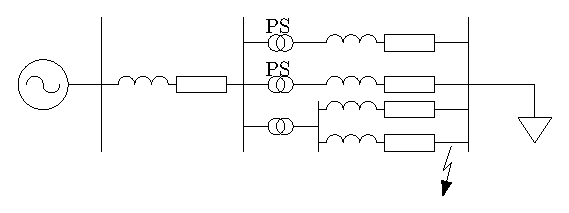
\includegraphics[width=0.8\textwidth]{PhaseShifters/PhaseShifters}
  \end{center}
  \caption{Illustration of the studied system}
\end{figure}

The line is disconnected at t = 30s.\\
Two simulations are done :
\begin{itemize}
\item the two phase shifters have the following time constants t1st = 40s/tNext = 20s;
\item one phase shifter have the following time constants t1st = 20s/tNext = 10s, the other one t1st = 40s/tNext = 20s.
\end{itemize}

The currents in both phase shifters are compared in both cases. One can observe that depending on the time constants of the phase shifter, the steady state after the event is different.\\
\\
This cannot be captured by a fully static simulator, in which all the phase shifters are activated at the same time with an external loop.

\begin{figure}[H]
  \begin{tikzpicture}
    \begin{axis}[xmin = 0, ymin = 0.24, ymax = 0.34, height = 2.3in, legend pos=north east]
        \addplot[color=red!50,line width=0.03in]
        table[x=time,y=PhaseShifter_5_6_phaseShifter_iMonitored]
        {PhaseShifters/curves2010.csv};
        \addplot[color=blue!50,line width=0.03in]
        table[x=time,y=PhaseShifter_5_6_phaseShifter_iMonitored]
        {PhaseShifters/curves4020.csv};
        \legend{20/10, 40/20}
        \end{axis}
  \end{tikzpicture}
  \caption{Current in the first phase shifter [pu]}
\end{figure}

\begin{figure}[H]
  \begin{tikzpicture}
    \begin{axis}[xmin = 0, ymin = 0.24, ymax = 0.34, height = 2.3in, legend pos=north east]
        \addplot[color=red!50,line width=0.03in]
        table[x=time,y=PhaseShifter_5_7_phaseShifter_iMonitored]
        {PhaseShifters/curves2010.csv};
        \addplot[color=blue!50,line width=0.03in]
        table[x=time,y=PhaseShifter_5_7_phaseShifter_iMonitored]
        {PhaseShifters/curves4020.csv};
        \legend{20/10, 40/20}
        \end{axis}
  \end{tikzpicture}
  \caption{Current in the second phase shifter [pu]}
\end{figure}

\section{Simplified HVDC link with AC emulation and phase shifter (HVDC\_PhaseShifter)}

The following system is simulated. It is made of a generator (GeneratorPVSignalN), a phase shifter transformer, four lines, two transformers, a simplified HVDC link with an AC emulation (SimplifiedHVDCACEmulation) and a PQ load (LoadPQ).\\

\begin{figure}[H]
  \begin{center}
  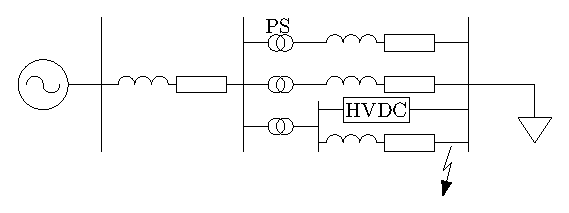
\includegraphics[width=0.8\textwidth]{HVDC_PhaseShifter/HVDC_PhaseShifter}
  \end{center}
  \caption{Illustration of the studied system}
\end{figure}

The line is disconnected at t = 30s.\\
Two simulations are done :
\begin{itemize}
\item the time constant of the HVDC link is equal to 50s;
\item the time constant of the HVDC link is equal to 1s.
\end{itemize}

One can observe that, in the case where the HVDC link time constant is equal to 50s, its power increases too slowly. As a consequence, the power in the phase shifter is too high for a too long time, which induces a tap change that doesn't happen when the time constant is equal to 1s.\\
\\
This cannot be captured by a fully static simulator, in which the HVDC link has no dynamics (which is equivalent to tFilter=0s).

\begin{figure}[H]
  \begin{tikzpicture}
    \begin{axis}[xmax = 120, height = 3in, legend pos=north east]
        \addplot[color=red!50,line width=0.03in]
        table[x=time,y=PhaseShifter_5_6_phaseShifter_PMonitored]
        {HVDC_PhaseShifter/curves1.csv};

        \addplot[color=blue!50,line width=0.03in]
        table[x=time,y=PhaseShifter_5_6_phaseShifter_PMonitored]
        {HVDC_PhaseShifter/curves50.csv};

        \legend{tFilter = 1s, tFilter = 50s}
        \end{axis}
  \end{tikzpicture}
  \caption{Active power in the phase shifter [pu]}
\end{figure}

\begin{figure}[H]
  \begin{tikzpicture}
    \begin{axis}[xmax = 120, height = 3in, legend pos=north east]
        \addplot[color=red!50,line width=0.03in]
        table[x=time,y=HVDC_hvdc_P1Pu]
        {HVDC_PhaseShifter/curves1.csv};

        \addplot[color=blue!50,line width=0.03in]
        table[x=time,y=HVDC_hvdc_P1Pu]
        {HVDC_PhaseShifter/curves50.csv};

        \legend{tFilter = 1s, tFilter = 50s}
        \end{axis}
  \end{tikzpicture}
  \caption{Active power in the HVDC link [pu]}
\end{figure}

\section{Simplified HVDC link with AC emulation and CLA (HVDC\_CLA)}

The following system is simulated. It is made of a generator (GeneratorPVSignalN), four lines (one is monitored by a current limiter automaton), two transformers, a simplified HVDC link with an AC emulation (SimplifiedHVDCACEmulation) and a PQ load (LoadPQ).\\

\begin{figure}[H]
  \begin{center}
  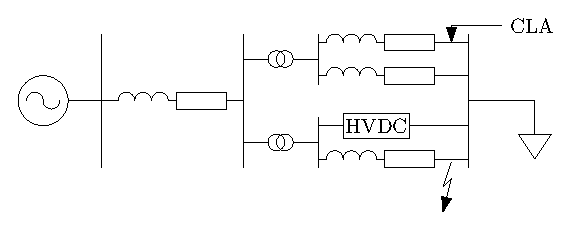
\includegraphics[width=0.8\textwidth]{HVDC_CLA/HVDC_CLA}
  \end{center}
  \caption{Illustration of the studied system}
\end{figure}

The line is disconnected at t = 30s.\\
Two simulations are done :
\begin{itemize}
\item the time constant of the HVDC link is equal to 60s;
\item the time constant of the HVDC link is equal to 30s.
\end{itemize}

One can observe that, in the case where the HVDC link time constant is equal to 60s, its power increases too slowly. As a consequence, the current in the line that is monitored by the CLA is too high for a too long time, which induces a line disconnection that doesn't happen when the time constant is equal to 30s.\\
\\
This cannot be captured by a fully static simulator, in which the HVDC link has no dynamics (which is equivalent to tFilter=0s).

\begin{figure}[H]
  \begin{tikzpicture}
    \begin{axis}[xmax = 120, height = 3in, legend pos=south east]
        \addplot[color=red!50,line width=0.03in]
        table[x=time,y=HVDC_hvdc_P1Pu]
        {HVDC_CLA/curves30.csv};

        \addplot[color=blue!50,line width=0.03in]
        table[x=time,y=HVDC_hvdc_P1Pu]
        {HVDC_CLA/curves60.csv};

        \legend{tFilter = 30s, tFilter = 60s}
        \end{axis}
  \end{tikzpicture}
  \caption{Active power in the HVDC link [pu]}
\end{figure}

\begin{figure}[H]
  \begin{tikzpicture}
    \begin{axis}[xmax = 120, height = 3in, legend pos=south east]
        \addplot[color=red!50,line width=0.03in]
        table[x=time,y=NETWORK__BUS____7-BUS___10-2_AC_iSide2]
        {HVDC_CLA/curves30.csv};

        \addplot[color=blue!50,line width=0.03in]
        table[x=time,y=NETWORK__BUS____7-BUS___10-2_AC_iSide2]
        {HVDC_CLA/curves60.csv};

        \legend{tFilter = 30s, tFilter = 60s}
        \end{axis}
  \end{tikzpicture}
  \caption{Current in the remaining AC line [A]}
\end{figure}

\section{Load restoration (LoadRestoration)}

The following system is simulated. It is made of a generator (GeneratorPVSignalN), two transformers, three lines and a restorative alpha beta load (LoadAlphaBetaRestorative).\\

\begin{figure}[H]
  \begin{center}
  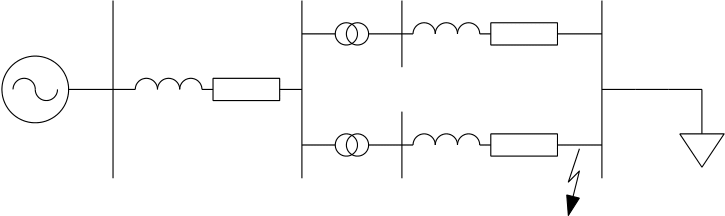
\includegraphics[width=0.8\textwidth]{LoadRestoration/LoadRestoration}
  \end{center}
  \caption{Illustration of the studied system}
\end{figure}

The line is disconnected at t = 30s.\\
Two simulations are done :
\begin{itemize}
\item the load restoration is complete (UMinPu = 0);
\item the load restoration is not complete (the voltage goes below UMinPu = 0.95 pu, which decreases the load active power following an alpha-beta behaviour).
\end{itemize}

One can notice that when the restoration is complete, the simulation fails, as would a purely static simulation (power flow).

When the restoration is not complete, the active power of the load is below the maximum transferrable power. As a consequence, the simulation succeeds.

\chapter{WSCC9}

The WSCC 9-bus system represents a simple approximation of the Western System Coordinating Council (WSCC) to an equivalent system with nine buses and three generators.
It was notably published in Anderson and Fouad’s book ‘Power System Control and Stability’ for the first time in 1980.

\section{Test case description}

The WSCC 9-bus system has 9 buses, 3 generators, 3 transformers, 6 lines and 3 loads.  \\
There are four voltage levels in the test case: 230 kV, 18 kV, 16.5 kV and 13.8 kV. The inner
part is the 230 kV part. The generators are at 18 kV, 16.5 kV and 13.8 kV.

\begin{figure}[H]
  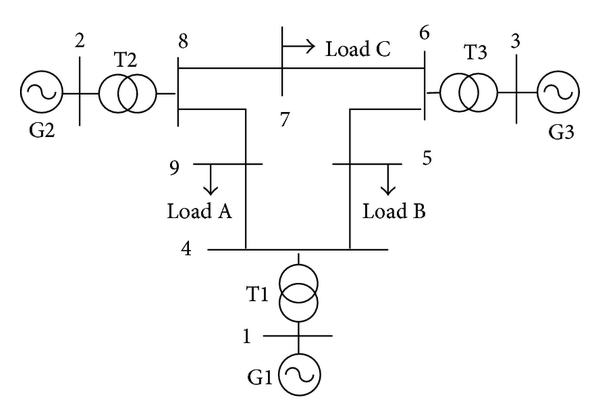
\includegraphics[width=\textwidth]{WSCC9Bus.jpg}
  \caption{WSCC 9-bus system diagram}
\end{figure}

\subsection{Initial Conditions}

The reference angle for the load flow is set at bus n°1. The initial conditions for each generator
are:
\begin{center}
\begin{tabular}{|c|c|c|c|c|}
  \hline
  Generator & P (MW) & Q (Mvar) & U (kV) & $\Theta$ (°) \\
  \hline
  1 & 71.94 & 24.05 & 15.60 & 0.00\\
  2 & 163.00 & 14.44 & 18.00 & 9.66\\
  3 & 85.00 & -3.65 & 13.80 & 4.77\\
  \hline
\end{tabular}
\end{center}

\subsection{Models}

\subsubsection{Synchronous machines}

All the generators are modeled as GeneratorPV: it means that they can adjust their Q to maintain the voltage equal to a target and their active power is modified by the frequency regulation model through the signal N variable.

\subsubsection{Loads}

Loads are modelled as restorative loads. After an event, the load goes back to its initial PPu/QPu unless the voltage at its terminal is lower than UMinPu or higher than UMaxPu. In this case, the load behaves as a classical Alpha-Beta load.

\subsection{Solver}
The solver used is a fixed Backward-Euler order 1 solver:
\begin{itemize}
\item $Time step$=10 s
\item $Tolerance$=$10^{-4}$
\end{itemize}

\subsection{Scenario}
The scenario simulated is the disconnection of the line between bus 1 and bus 5.

\newpage
\section{Results}

Here are the final values obtained for each generator:

\begin{center}
\begin{tabular}{|c|c|c|c|c|}
  \hline
  Generator & P (MW) & Q (Mvar) & U (kV) & $\Theta$ (°) \\
  \hline
  1 & 70.98 & 20.98 & 15.60 & 0.00\\
  2 & 161.85 & 18.72 & 18.00 & 5.15\\
  3 & 83.96 & 17.53 & 13.80 & -2.69\\
  \hline
\end{tabular}
\end{center}

And the final power flows on the lines:

\begin{center}
\begin{tabular}{|c|c|c|c|c|}
  \hline
  Line & $P_{Or} (MW)$ & $P_{Ex} (MW)$ & $Q_{Or} (Mvar)$ & $Q_{Ex} (Mvar)$ \\
  \hline
  Bus4-Bus5 & 70.98 & -70.40 & 17.82 & -29.55 \\
  Bus5-Bus7 & -54.59 & 55.64 & -20.44 & -3.50 \\
  Bus6-Bus9 & -85.71 & -27.65 & 89.17 & 10.02 \\
  Bus7-Bus8 & 106.21 & -105.22 & 5.64 & -11.76 \\
  Bus8-Bus9 & 5.22 & -5.19 & -23.23 & 3.19 \\
  \hline
\end{tabular}
\end{center}

\chapter{IEEE14}

The IEEE 14-bus system is a standard test case in the power system community. It represents a simple approximation of the American Electric Power system (in the U.S. Midwest) as it was in the early 1960s. The data were provided by Iraj Dabbagchi of AEP and converted into the IEEE Common Data Format by Rich Christie at the University of Washington in August 1993.

\textbf{Note. The test case is used in a modified way in this example: arbitrary data are added to the test case and synchronous condensers 3, 6 and 8 are considered as classical synchronous machines (their active power can be different from zero).}

% Generic description of the non regression test
% List of scenarios
\section{Test case description}

The IEEE 14-bus test case system has 14 buses, 5 generators, 1 shunt, 3 transformers, 16 lines and 11 loads.\\
There are two voltage levels in the test case: 69 kV and 13.8 kV. The lower part of the system, with generators 1, 2 and 3, corresponds to the 69 kV network, whereas the upper part is the 13.8 kV network.

\begin{figure}[H]
  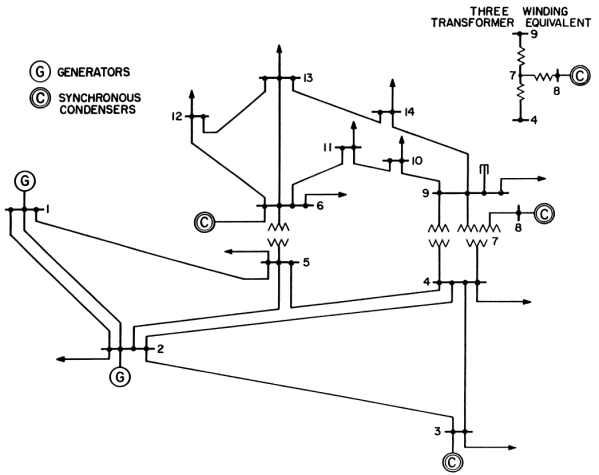
\includegraphics[width=\textwidth]{Single-line-diagram-of-IEEE-14-bus-system.png}
  \caption{IEEE 14 bus system diagram}
\end{figure}

\subsection{Initial Conditions}

The reference angle for the load flow is set at bus n°1. \\

Here are the initial conditions for each generator.

\begin{center}
\begin{tabular}{|c|c|c|c|c|}
  \hline
  Generator & P (MW) & Q (Mvar) & U (kV) & $\Theta$ (°) \\
  \hline
  1 & 232.39 & -16.55 & 73.14 & 0.00\\
  2 & 40.00 & 43.56 & 72.11 & -4.98\\
  3 & 0.00 & 25.07 & 69.69 & -12.73\\
  6 & 0.00 & 12.73 & 14.77 & -14.22\\
  8 & 0.00 & 17.62 & 15.04 & -13.36\\
  \hline
\end{tabular}
\end{center}

\subsection{Models}

\subsubsection{Synchronous machines}

All the generators and the synchronous condensers are modeled as GeneratorPV: it means that they can adjust their Q to maintain the voltage equal to a target and their active power is modified by the frequency regulation model through the signal N variable.

\subsubsection{Loads}

Loads are modelled as restorative loads. After an event, the load goes back to its initial PPu/QPu unless the voltage at its terminal is lower than UMinPu or higher than UMaxPu. In this case, the load behaves as a classical Alpha-Beta load.

\subsection{Solver}
The solver used is a fixed Backward-Euler order 1 solver:
\begin{itemize}
\item $Time step$=10 s
\item $Tolerance$=$10^{-4}$
\end{itemize}

\subsection{Scenario}
The scenario simulated is the disconnection of the line between bus 1 and bus 5.

\newpage
\section{Results}

\textbf{As a remainder, synchronous condensers are considered as normal synchronous machines in the current set of data: their active power can thus vary}. \\

Here are the final values obtained for each generator:

\begin{center}
\begin{tabular}{|c|c|c|c|c|}
  \hline
  Generator & P (MW) & Q (Mvar) & U (kV) & $\Theta$ (°) \\
  \hline
  1 & 234.46 & -36.84 & 73.14 & 0.00\\
  2 & 41.92 & 74.70 & 72.11 & -4.97\\
  3 & 2.82 & 28.80 & 69.69 & -12.73\\
  6 & 0.14 & 21.14 & 14.77 & -14.22\\
  8 & 0.43 & 19.84 & 15.04 & -13.36\\
  \hline
\end{tabular}
\end{center}

And the final power flows on the lines:

\begin{center}
\begin{tabular}{|c|c|c|c|c|}
  \hline
  Line & $P_{Or} (MW)$ & $P_{Ex} (MW)$ & $Q_{Or} (Mvar)$ & $Q_{Ex} (Mvar)$ \\
  \hline
  Bus1-Bus2 & 156.77 & -152.48 & -20.5 & 27.76 \\
  Bus1-Bus5 & 75.51 & -72.74 & 3.85 & 2.22 \\
  Bus2-Bus3 & 73.32 & -71 & 3.58 & 1.59 \\
  Bus2-Bus4 & 56.17 & -54.5 & -1.5 & 3 \\
  Bus2-Bus5 & 41.55 & -40.65 & 1.2 & -2.2 \\
  Bus3-Bus4 & -23.33 & 23.7 & 4.5 & -4.85 \\
  Bus4-Bus5 & -61.16 & 61.67 & 15.82 & -14.2 \\
  Bus6-Bus11 & 7.42 & -7.36 & 3.68 & -3.56 \\
  Bus6-Bus12 & 7.84 & -7.76 & 2.6 & -2.44 \\
  Bus6-Bus13 & 17.86 & -17.64 & 7.4 & -6.97 \\
  Bus9-Bus10 & 5.22 & -5.21 & 2.6 & -2.44 \\
  Bus9-Bus11 & 9.26 & -9.15 & 3.25 & -3 \\
  Bus10-Bus11 & -3.78 & 3.79 & -1.61 & 1.64 \\
  Bus12-Bus13 & 1.61 & -1.61 & 0.75 & -0.74 \\
  Bus13-Bus14 & 5.5 & -5.46 & 1.46 & -1.36 \\
  \hline
\end{tabular}
\end{center}

\end{document}
